\documentclass{article}
% \synctex=1
% \newcommand{\fix}[1]{{\bf *** #1 ***}}
\usepackage{amsfonts, amsmath, comment, hyperref, fontawesome5}
\usepackage{mathrsfs, amssymb, tikz-cd, booktabs}
\usepackage{stmaryrd, siunitx, lmodern, multicol, adjustbox}
\usepackage{multirow, pifont, soul, enumerate}
\usepackage{latexsym, cancel, xcolor, url, color}
\usepackage{listings, amsthm}
\usepackage{imakeidx}
\usepackage[ruled,linesnumbered,boxruled,slide]{algorithm2e}
\usepackage[symbol]{footmisc}
\usepackage{textcomp}
\usepackage[T1]{fontenc}
\usepackage{marvosym}
\usepackage{harmony}
\usepackage{hieroglf}
\usepackage[noend]{algpseudocode}
\usepackage{colortbl}
\usepackage{wasysym}
\usepackage{tikz}
\usetikzlibrary{automata, positioning}

\hypersetup{
    colorlinks,
    linkcolor={red!50!black},
    citecolor={blue!50!black},
    urlcolor={blue!80!black}
}

\usepackage[OT2,OT1]{fontenc}
\def\SH{\mbox{\fontencoding{OT2}\selectfont\char88}}

\newcommand\blfootnote[1]{%
    \begingroup
    \renewcommand\thefootnote{}\footnote{#1}%
    \addtocounter{footnote}{-1}%
    \endgroup
}

\linespread{1.2} 

\usepackage[all]{xy}
\usetikzlibrary{calc}
\usetikzlibrary{shapes, positioning}
\tikzset{
	arr/.style={-stealth,shorten >=4.2mm,shorten <=4.2mm,thick}, %
	dot/.style={rotate=-45,font=\LARGE}, %
	dot2/.style={rotate=45,font=\LARGE} %
}

\usepackage{amssymb}
\usepackage[many]{tcolorbox}
\newtcolorbox[auto counter,number within=section]{Question}[2][]{%
    colback=green!5,
    colframe=green!35!black,
    colbacktitle=green!35!black,
    coltitle=white,
    fonttitle=\bfseries, 
    title=Question~\thetcbcounter.\ #2,
    enhanced,
    attach boxed title to top left={yshift=-2mm, xshift=0.5cm},%
    #1% 
}

\lstset{
    basicstyle=\ttfamily, % Set the default font for listings to typewriter
    mathescape=true,      % Allows escaping to LaTeX math mode within $$
    columns=fullflexible,
    breaklines=true,      % Set automatic line breaking
    captionpos=b,         % Sets the caption-position to bottom
    xleftmargin=\parindent,
    numbers=left,         % Line numbers on left
    numberstyle=\small,   % Line numbers styling
    numbersep=5pt,
    escapeinside={(*@}{@*)} % for escaping to LaTeX inside your code
}

\setlength{\textheight}{8.75in}
\setlength{\textwidth}{6.5in}
\setlength{\topmargin}{0.0in}
\setlength{\headheight}{0.0in}
\setlength{\headsep}{0.0in}
\setlength{\leftmargin}{0.0in}
\setlength{\oddsidemargin}{0.0in}
\setlength{\parindent}{3pc}

\newenvironment{solution}[1][\proofname]{
    \proof[\textbf{Solution:}] \renewcommand{\qedsymbol}{$\bell$}
}{\endproof}

\begin{document}

\begin{center}
    Solution to Exercises
\end{center} 

% *
% !
% ?
% TODO 
% FIXME: 
% // 

\noindent \textbf{Exercise 3.1}: 

\begin{solution}

\end{solution}

\noindent \textbf{Exercise 5.1}: 

\begin{solution}
    Suppose for a contradiction that $L$ is a regular language, thus there exists pumping length $p$ satisfying the pumping lemma. Now consider the string 
    \[ \omega := 0^p 1^p \in L \]
    of length $2p$. For this string, in its decomposition $\omega = xyz$, we have $xy$ is made of purely zero's. In particular, $y$ consists of only zero's. It is now easy to see that 
    \[ x y^i z \notin L \]
    for, for example, $i = 2$. This contradicts our assumption that $L$ is regular, hence $L$ is not regular. 
\end{solution}

\noindent \textbf{Exercise 5.2} \label{exercise5.2}: 

\begin{solution}
    Since we have the convention that $(0)_k$ is the empty word, we have the following automoton accepting the set: \begin{center}
        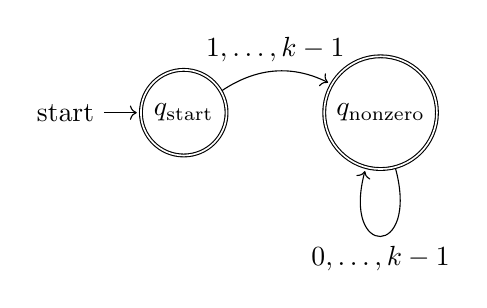
\begin{tikzpicture}[shorten >=1pt, node distance=2.5cm, on grid, auto]
            \node[state, initial, accepting] (q0) {$q_{\text{start}}$};
            \node[state, accepting] (q1) [right=of q0] {$q_{\text{nonzero}}$};
        
            % Transitions
            \path[->]
            (q0) edge[bend left] node[above] {$1,\dots,k-1$} (q1)
            (q1) edge[loop below] node {$0,\dots,k-1$} ()
            ;
        \end{tikzpicture}
    \end{center}
\end{solution}

\noindent \textbf{Exercise 5.3} \label{exercise5.3}: 

\begin{solution}
    % ¹²³⁴⁵⁶⁷⁸⁹⁰
    % suppose we have k = 10 and w = 1111, u = 2, v = 5
    % now we have   [uw]ₖ   =   21111 = 𝛼 10⁰ + 𝛽 
    %               [uvw]ₖ  =  251111 = 𝛼 10¹ + 𝛽 
    %               [uv²w]ₖ = 2551111 = 𝛼 10² + 𝛽 

    % suppose we have k = 2 and w = 3, u = 2, v = 5
    % now we have   [uw]ₖ   =  7 = 𝛼 2⁰ + 𝛽 
    %               [uvw]ₖ  = 21 = 𝛼 2¹ + 𝛽 
    %               [uv²w]ₖ = 59 = 𝛼 2² + 𝛽 

    Recall that we know for $\omega = d_m d_{m-1} \cdots d_0$, we have defined 
    \[ [\omega]_k = d_m k^m + d_{m-1} k^{m-1} + \cdots + d_1 k + d_0 \]
    Thus we can extend this definition and find that in general, we have 
    \begin{align*}
        [u v^n \omega]_k 
        & = [u]_k \cdot k^{n|v| + |\omega|} + [v]_k \cdot (1 + k^{|v|} + \cdots + k^{(n-1)|v|}) k^{|\omega|} + [\omega]_k \\ 
        & = [u]_k \cdot k^{n|v| + |\omega|} + [v]_k \cdot k^{|\omega|} \cdot \frac{k^{n|v|} - 1}{k^{|v|} - 1} + [\omega]_k \\ 
        & = \underbrace{ \left( [u]_k \cdot k^{|\omega|} + \frac{[v]_k \cdot k^{|\omega|}}{k^{|v|} - 1} \right) k^{|v|} }_{\alpha} \cdot k^{n} + \underbrace{ \left( - \frac{1}{k^{|v|} - 1} + [\omega]_k \right) }_{\beta} 
    \end{align*}
    the result is now obvious. 
\end{solution}

\noindent \textbf{Exercise 5.4} \label{exercise5.4}: 

\begin{solution}
    Similar to exercise 5.1 with the use of Fermat's Little Theorem. Suppose for a contradiction that the set $S$ is regular, thus it needs to satisfy the pumping lemma for some pumping length $p$. Find a prime $\gamma$ 
\end{solution}

\noindent \textbf{Exercise 5.5} \label{exercise5.5}: 

\begin{solution}
    This is similar to exercise 5.1. Suppose for a contradiction that the set of palindromes is regular, then there exists a pumping length $p$ satisfying the pumping lemma. Now consider an arbitrary string $\omega$ (palindrome) of length $2p + 1$, we know that in the decomposition $\omega xyz$, $xy$ does not contain the middle character of the palindrome $\omega$. As a result, it is now easy to see that the new string 
    \[ x y^i z \]
    wouldn't be a palindrome as desired, which further implies that $x y^i z \notin L$. This contradicts the pumping lemma, which means that that $L$ is not regular. 
\end{solution}




\end{document}